\documentclass[11pt,a4paper]{article}

%, , , , , , , , , , , , , , , , , , , , , , , , , -
%  Smart Multi-Level Parking Optimization -- project report
%  Compile with: pdflatex report.tex  (run twice for the table of contents)
%  Figures are read from the viz/ folder produced by main.ipynb.
%, , , , , , , , , , , , , , , , , , , , , , , , , -

\usepackage[utf8]{inputenc}
\usepackage[T1]{fontenc}
\usepackage{lmodern}
\usepackage[a4paper,margin=2.4cm]{geometry}
\usepackage{amsmath,amssymb}
\usepackage{graphicx}
\usepackage{booktabs}
\usepackage{array}
\usepackage{caption}
\usepackage{subcaption}
\usepackage{xcolor}
\usepackage{enumitem}
\usepackage{algorithm}
\usepackage{algpseudocode}
\usepackage{fancyhdr}
\usepackage{titlesec}
\usepackage[hidelinks]{hyperref}

\graphicspath{{viz/}}

\definecolor{accent}{RGB}{44,82,130}
\definecolor{lightgray}{RGB}{240,240,240}

\titleformat{\section}{\Large\bfseries\color{accent}}{\thesection}{0.7em}{}
\titleformat{\subsection}{\large\bfseries}{\thesubsection}{0.6em}{}

\pagestyle{fancy}
\fancyhf{}
\lhead{\small Smart Multi-Level Parking Optimization}
\rhead{\small Project 4 - Combinatorial Optimization \& Metaheuristics}
\cfoot{\thepage}
\renewcommand{\headrulewidth}{0.4pt}

\newcommand{\code}[1]{\texttt{\small #1}}

\begin{document}

% ============================== TITLE ==============================
\begin{titlepage}
\centering
\vspace*{2.5cm}
{\color{accent}\rule{\textwidth}{1.5pt}}\\[0.6cm]
{\Huge\bfseries Smart Multi-Level Parking Optimization}\\[0.5cm]
{\Large An Online Min-Cost Assignment Approach}\\[0.3cm]
{\color{accent}\rule{\textwidth}{1.5pt}}\\[1.4cm]

{\large\itshape Project 4 - Combinatorial Optimization \& Metaheuristics}\\[2.5cm]

{\large\bfseries Team}\\[0.4cm]
{\large Houaria Djabir \quad$\cdot$\quad Yasmine Meriche \quad$\cdot$\quad Nacer Eddine Missouni}\\[3cm]

{\large\today}
\vfill
\end{titlepage}

% ============================== TOC ==============================
\tableofcontents
\thispagestyle{fancy}
\newpage

% ============================== 1. INTRODUCTION ==============================
\section{Introduction and Problem Statement}

Cars arrive at a multi-level car park throughout the day, and each car must be
given a parking bay \emph{the moment it arrives}. The operator wants to serve the
demand as well as possible: park as many cars as physically possible and, among the
parked cars, keep the total \emph{inconvenience} low. Inconvenience is a deliberately
broad notion. It includes the walking distance from the bay to the exit, an electric
vehicle (EV) that fails to get a charging bay, a long-staying staff member occupying
a prime near-exit spot that a short-stay visitor needed, a small car wasting a scarce
large bay, and the crowding of one floor while other levels stay empty.

The single most important characteristic of this problem, the one that shapes every
design decision in the project, is that the system is \textbf{online}. We do not have
the luxury of seeing the whole day at once and computing a globally optimal schedule.
Instead, decisions arrive as a stream and must be committed immediately and
irrevocably. The remainder of this section makes the model precise; the following
sections describe the data, the shared cost function, the six solution methods, the
simulation engine, the experimental results, and their interpretation.

\subsection{The constraints}

The model respects six constraints, listed here in the order of their consequence for
the algorithm design:

\begin{description}[leftmargin=1.4em,style=nextline]
  \item[Online.] At minute $t$ we only know the cars that have \emph{already} arrived.
        We never observe future arrivals.
  \item[Unknown duration.] The decision policy does not know how long a car will stay.
        A bay becomes free only when its car actually leaves. The simulation
        \emph{environment} knows the true departure time (it must, to release bays), but
        this information is hidden from the decision method.
  \item[Irrevocable.] Once a car is parked it cannot be moved to another bay.
  \item[Simultaneity.] Cars that arrive in the same minute are all standing at the gate
        at the same instant, so they are decided \emph{together} and matched to the bays
        that are free at that moment.
  \item[Size rule (hard).] A \emph{Large} car can only use a \emph{Large} bay. Compact
        and Standard cars fit any bay. This is the one inviolable feasibility constraint.
  \item[One car per bay.] A bay holds exactly one car until that car leaves; it can then
        be reused.
\end{description}

\subsection{Why the problem reduces to a per-minute assignment}

Because several cars frequently arrive in the same minute, and because no method may
look into the future or reason about durations, the genuine decision faced at every
instant is a \textbf{min-cost assignment} of \emph{that minute's} arriving cars to the
bays that are free \emph{right now}. There is no interval reasoning, no look-ahead over
future arrivals, no duration-aware packing, those would all violate the online
constraint. This reduction is the conceptual backbone of the whole project: a hard
online sequential decision problem is decomposed into a sequence of small, well-defined
combinatorial assignment problems, one per minute, each of which the six methods solve
in a different way. The only forward-looking component permitted is a lightweight
\emph{anticipation} signal built purely from the history already observed, used by one
method (Section~\ref{sec:methods}).

% ============================== 2. DATA ==============================
\section{Data and Exploratory Analysis}

\subsection{The vehicle stream}

The demand is a fixed set of 1000 cars stored in \code{data/vehicles.csv}. Each car
record carries its type (Compact, Standard or Large), an EV flag, a user type (Staff or
Visitor), and an arrival and departure minute-of-day. The departure is used only by the
environment to release bays; the policy never sees it.

This vehicle set was derived from a public IIoT smart-parking dataset
(\code{IIoT\_Smart\_Parking\_Management.csv}) by the preparation notebook
\code{data/data\_prep.ipynb}. The derivation:
\begin{itemize}[leftmargin=1.4em]
  \item maps the source vehicle weight to a size class (Compact $\le 1200$\,kg,
        Standard $\le 1800$\,kg, Large $>1800$\,kg);
  \item normalises the user type, a record is \emph{Staff} if it was already marked
        Staff or if its parking duration is at least 7 hours, otherwise \emph{Visitor}, which is what gives staff their characteristic long stays;
  \item synthesises arrival times that follow a realistic non-residential profile:
        10\,\% of arrivals in 07:00--11:00, 60\,\% in 11:00--17:00, and 30\,\% in
        17:00--23:00, with 1--5 minute inter-arrival spacing inside each band, and longer
        stays scheduled earlier so that all departures fall before 23:00.
\end{itemize}

\subsection{The ten car parks}

Ten candidate car-park layouts are stored as \code{data/parking1.json} \dots
\code{parking10.json}. They range from 98 to 486 bays across 1 to 4 floors. Each bay
declares its floor, size (Small or Large), a charger flag, and a distance to the exit.
At load time we additionally tag the bottom 25\,\% nearest bays as ``near exit''. The
loaders build the two core data structures used everywhere in the code:

\begin{center}
\begin{tabular}{@{}ll@{}}
\toprule
\code{Car} & \code{id, v\_type, is\_ev, user\_type, arrival, departure} \\
\code{Bay} & \code{id, floor, size, has\_charger, near\_exit, distance\_to\_exit} \\
\bottomrule
\end{tabular}
\end{center}

\subsection{Demand profile and the capacity ceiling}

Figure~\ref{fig:demand} shows the four faces of the demand. Arrivals peak in the midday
band; durations are heavily right-skewed (most cars stay a short while, a minority stay
all day); the fleet is dominated by Compact and Standard cars with a Large minority; and
EVs and Staff are both minorities (EVs around 20\,\%, Staff only 51 of the 1000 cars).

\begin{figure}[h]
  \centering
  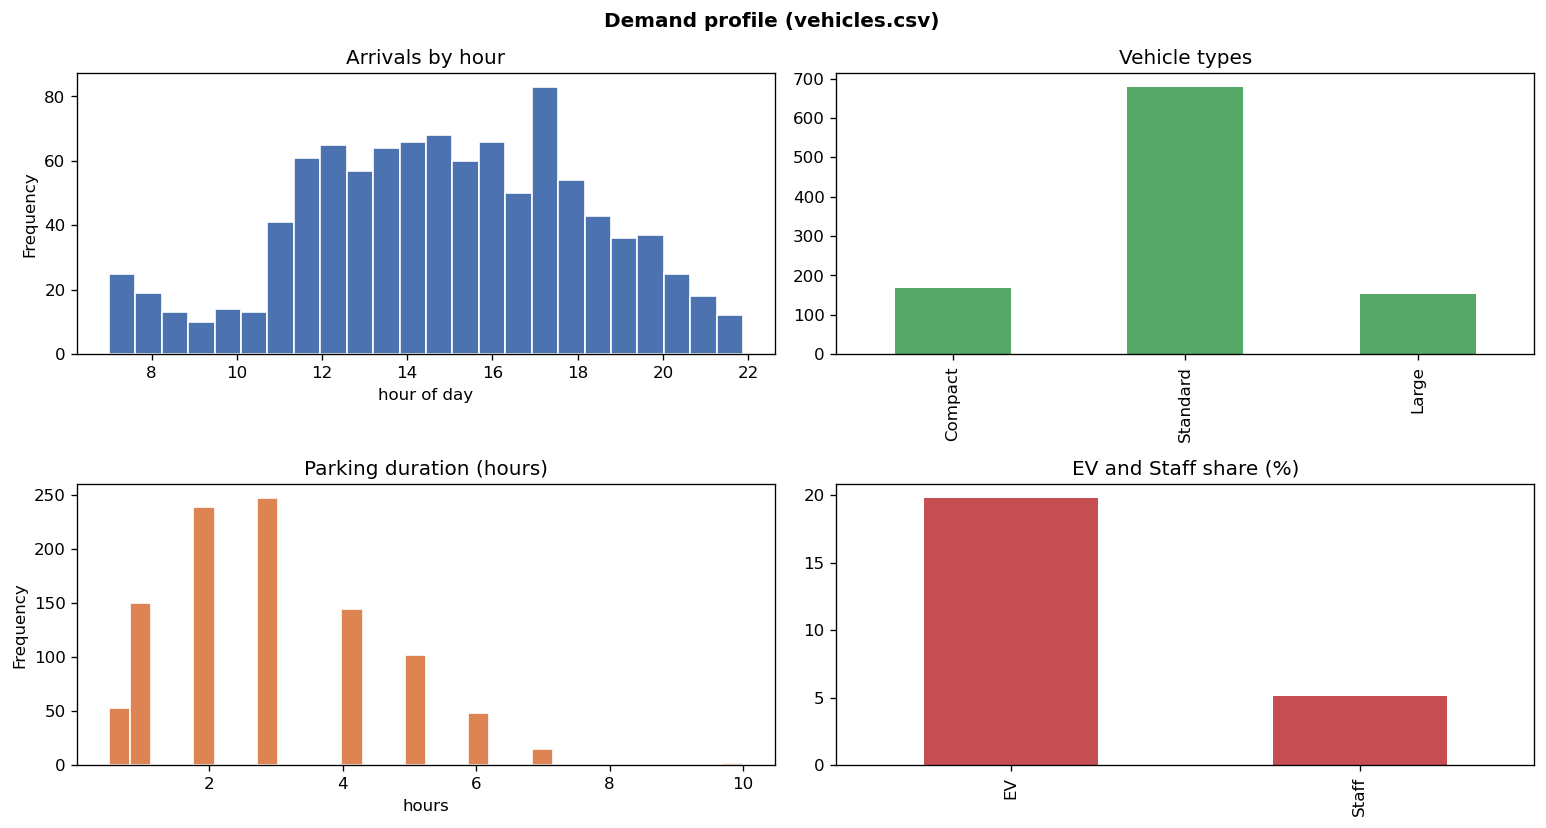
\includegraphics[width=0.92\textwidth]{mt_demand.png}
  \caption{Demand profile of the 1000-car stream: arrivals by hour, vehicle-type mix,
           parking-duration distribution, and the EV / Staff shares.}
  \label{fig:demand}
\end{figure}

A single number governs how many cars can ever be parked: the \emph{peak concurrent
demand}, obtained by sweeping the arrival/departure events and tracking how many cars
are simultaneously present. That peak is \textbf{355 cars at once}.
Figure~\ref{fig:capacity} compares each park's capacity against this line. Three parks
(3, 8 and 10) have fewer than 355 bays, so they physically cannot hold everyone at the
peak, no matter how clever the policy. This single fact explains why every method will
later park almost exactly the same fraction of cars: capacity sets the headline number,
and the method only sets the \emph{quality} of the placements.

\begin{figure}[h]
  \centering
  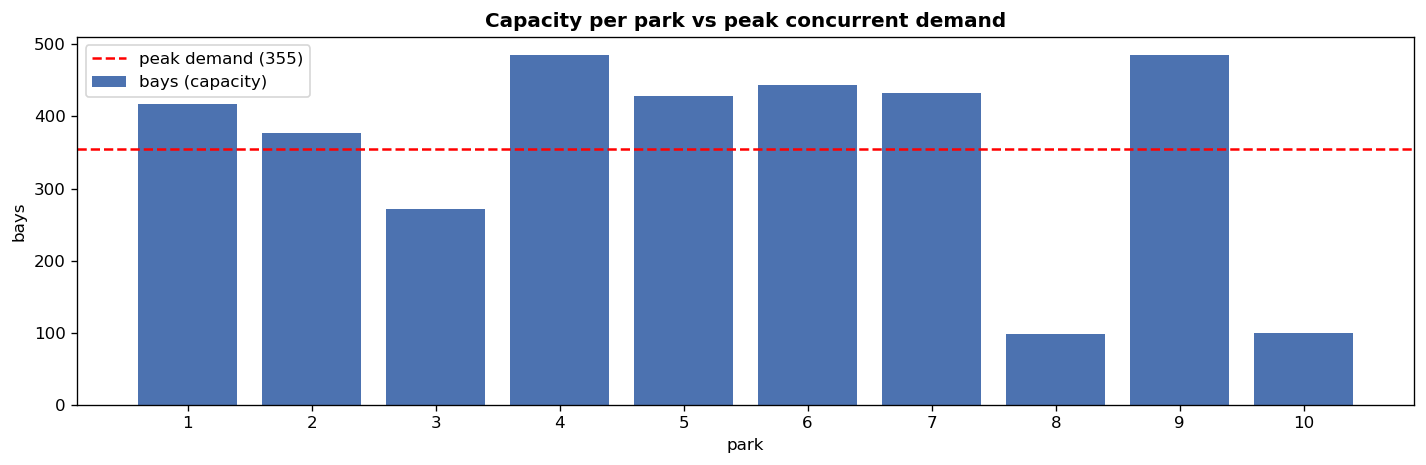
\includegraphics[width=0.92\textwidth]{mt_capacity.png}
  \caption{Capacity (bays) per park versus the peak concurrent demand of 355 cars.
           Parks below the dashed line saturate at peak.}
  \label{fig:capacity}
\end{figure}

% ============================== 3. COST FUNCTION ==============================
\section{The Shared Cost Function}
\label{sec:cost}

Every method minimises the \emph{same} cost when it matches a car to a bay. Centralising
the objective in one function is what makes the six methods comparable: they differ only
in \emph{how} they search for the minimum, never in \emph{what} they consider good. The
cost is deliberately \emph{scarcity-aware}, it does not merely look at the car in
front of us, it also protects the bays that are scarce and valuable.

For a car $c$ placed in bay $b$, let $d$ be the bay's distance to the exit and
$D_{\max}$ the farthest distance in the park. The cost is
\begin{equation}
\label{eq:cost}
\begin{aligned}
\mathrm{cost}(c,b) \;=\;
&\underbrace{\Big[\,\mathbf{1}[c\text{ is Staff}]\,(D_{\max}-d) + \mathbf{1}[c\text{ is Visitor}]\,d\,\Big]}_{\text{access term (staff pushed to the back)}}
\;+\; \underbrace{w_{\text{fl}}\,(\mathrm{floor}(b)-1)}_{\text{upper-floor penalty}} \\[4pt]
&+\; \underbrace{p_{\text{ev}}\,\mathbf{1}[c\text{ is EV} \wedge b\text{ has no charger}]}_{\text{EV without a charger}}
\;+\; \underbrace{c_w\,\mathbf{1}[b\text{ has a charger} \wedge c\text{ not EV}]}_{\text{charger preservation}} \\[4pt]
&+\; \underbrace{s_w\,\mathbf{1}[b\text{ is Large} \wedge c\text{ not Large}]}_{\text{large-bay preservation}}
\;+\; \underbrace{f_{\text{ld}}\cdot \rho_{\mathrm{floor}(b)}}_{\text{floor load balancing}}
\end{aligned}
\end{equation}
where $\rho_{\mathrm{floor}(b)}$ is the current occupancy fraction of the chosen floor.
Each term encodes one piece of the inconvenience notion from Section~1:

\begin{description}[leftmargin=1.4em,style=nextline]
  \item[Walking distance.] The base inconvenience for a visitor is simply $d$.
  \item[The staff flip.] Staff stay long, so for a staff car the access cost is
        $D_{\max}-d$ instead of $d$. This deliberately pushes long-stay staff to the
        \emph{back} of the park, freeing the prime near-exit bays for the many short-stay
        visitors who churn through them. Visitors keep the natural $d$, so they prefer
        near bays.
  \item[Floor penalty.] Upper floors cost $w_{\text{fl}}$ per level above the ground,
        since reaching them takes longer.
  \item[EV needs a charger.] A large penalty $p_{\text{ev}}$ if an electric car is placed
        without a charger.
  \item[Charger preservation.] A penalty $c_w$ if a non-EV takes a charger bay, so that
        scarce chargers stay free for EVs.
  \item[Large-bay preservation.] A penalty $s_w$ if a non-large car takes a large bay, so
        that scarce large bays stay free for large cars.
  \item[Floor load balancing.] A mild penalty proportional to how full the chosen floor
        already is, which spreads cars across levels.
\end{description}

All weights are tunable constants declared at the top of the notebook
(Table~\ref{tab:weights}). The two \emph{preservation} terms ($c_w$ and $s_w$) are the
only ones the anticipation module rescales, and only for one method.

\begin{table}[h]
  \centering
  \caption{Tunable cost weights (units: metres-equivalent; raw distance is $\sim$5--60\,m).}
  \label{tab:weights}
  \begin{tabular}{@{}llr@{}}
    \toprule
    Symbol & Constant & Value \\
    \midrule
    $p_{\text{ev}}$  & \code{EV\_PEN}        & 80.0 \\
    $c_w$            & \code{CHARGER\_WASTE} & 25.0 \\
    $s_w$            & \code{SIZE\_WASTE}    & 25.0 \\
    $w_{\text{fl}}$  & \code{W\_FLOOR}       & 15.0 \\
    $f_{\text{ld}}$  & \code{FLOOR\_LOAD}    & 20.0 \\
    $\lambda$        & \code{LAMBDA} (anticipation) & 3.0 \\
    --               & \code{UNASSIGNED}     & $10^{6}$ \\
    \bottomrule
  \end{tabular}
\end{table}

Leaving a car unparked is modelled by a sentinel cost \code{UNASSIGNED}~$=10^6$, which
dwarfs any real placement cost. The optimiser therefore parks a car whenever a feasible
bay exists, and only ever ``chooses'' to leave a car on the street when the park is
genuinely full. This single trick lets the same min-cost machinery handle both the
quality objective and the capacity constraint at once.

% ============================== 4. METHODS ==============================
\section{The Six Solution Methods}
\label{sec:methods}

Every minute we must match the cars that just arrived to the bays free right now, at
minimum total cost. That is a min-cost assignment problem, and the six methods are six
different ways to solve it. The first is a naive baseline; the next three are exact; the
last two are metaheuristics.

\subsection{Shared scaffolding}

Two helpers are shared by all the joint solvers. The \code{compatible} test enforces the
single hard size rule. The \code{\_pool} helper restricts the search to a small candidate
set: for a group of $g$ cars it gathers, for each car, its $g+5$ cheapest compatible free
bays and takes the union. The optimal matching of $g$ cars never needs more bays than
this, so the candidate pool keeps every solver's search tiny without sacrificing
optimality. Single-car minutes (the common case) bypass the machinery entirely and just
take the cheapest compatible bay.

\subsection{Baseline, greedy nearest bay}

Each car, one at a time, takes the nearest free compatible bay, using distance
\emph{only}. There is no joint matching and none of the scarcity terms. This is the
obvious, naive approach and the yardstick everything else is measured against.

\subsection{ILP, exact integer program}

The matching is written as a binary program with variables $x_{c,b}\in\{0,1\}$ and solved
exactly by CBC through \code{pulp}:
\begin{align}
\min \quad & \sum_{c,b} \mathrm{cost}(c,b)\,x_{c,b}
           + \sum_{c}\mathrm{UNASSIGNED}\Big(1-\sum_{b}x_{c,b}\Big) \\
\text{s.t.}\quad & \sum_{b} x_{c,b} \le 1 \quad \forall c
           \qquad\text{(each car at most one bay)}\\
           & \sum_{c} x_{c,b} \le 1 \quad \forall b
           \qquad\text{(each bay at most one car)}
\end{align}
This is the formal, declarative statement of the problem and the exact reference the
others are checked against. \code{pulp} is an optional dependency: if it is absent every
ILP step is skipped and Branch \& Bound remains as the exact reference.

\subsection{B\&B, branch and bound}

A depth-first search over the cars that assigns each car to a bay or leaves it unparked,
pruning any branch whose accumulated cost plus an admissible suffix lower bound already
meets or exceeds the best solution found so far. It is warm-started with a greedy
matching and bounded by a time limit (2\,s). It reaches the same optimum as ILP, by
explicit search rather than by a solver.

\subsection{SA, simulated annealing}

A metaheuristic local search that starts from a greedy matching and improves it with
small moves, reassign one car to a different free bay, or swap two cars' bays, accepting worse moves with the usual Metropolis probability $\exp(-\Delta/T)$ to escape
local minima. The temperature cools geometrically and the iteration budget scales with
the minute size ($\min(1500, 40g)$). It approximates the optimum.

\subsection{GA, genetic algorithm}

A metaheuristic that evolves a population of matchings. Each chromosome maps cars to
bays; tournament selection, one-point crossover and swap mutation produce offspring, and
a repair step guarantees that no two cars share a bay. Elitism preserves the two best
individuals each generation. Population and generation counts scale with the minute size.
It too approximates the optimum.

\subsection{Hungarian, Kuhn--Munkres with anticipation}

The Kuhn--Munkres algorithm solves the assignment problem exactly in $O(n^3)$. The cost
matrix has one row per car and one column per candidate bay, plus $g$ extra ``street''
columns of cost \code{UNASSIGNED} that let a car stay unparked; incompatible cells are
set above \code{UNASSIGNED} so they are never chosen. Crucially, Hungarian is the only
method carrying an \textbf{always-on anticipation} signal. Using the arrivals seen so far
and the current scarcity of chargers and large bays, it scales the two preservation
weights
\begin{equation}
c_w = \mathrm{CHARGER\_WASTE}\,(1+\lambda\,p_{\text{ev}}\,\rho_{\text{ch}}), \qquad
s_w = \mathrm{SIZE\_WASTE}\,(1+\lambda\,p_{\text{lg}}\,\rho_{\text{lg}}),
\end{equation}
where $p_{\text{ev}},p_{\text{lg}}$ are the observed EV and large-car fractions and
$\rho_{\text{ch}},\rho_{\text{lg}}$ the current occupancy of charger and large bays. When
chargers are filling up and the history says EVs keep coming, the penalty for letting a
non-EV waste a charger rises, so Hungarian reserves those scarce bays for the high-need
cars still to arrive. This look-ahead uses only past observations, it never peeks at
future arrivals, so it honours the online constraint.

\begin{algorithm}[h]
\caption{One minute, the Hungarian method}
\label{alg:hungarian}
\begin{algorithmic}[1]
\State \textbf{Input:} arriving group, free bays, $D_{\max}$, floor occupancy, weights $c_w,s_w$
\If{group has one car} \Return its cheapest compatible bay \EndIf
\State pool $\gets$ union of each car's $g{+}5$ cheapest compatible bays
\State build cost matrix $M$ (cars $\times$ [pool $\cup$ street columns])
\State assign $\gets$ \textsc{KuhnMunkres}($M$)
\State \Return for each car, its assigned pool bay, or \textbf{None} if a street column was chosen
\end{algorithmic}
\end{algorithm}

\paragraph{A note on fair comparison.} ILP, B\&B and Hungarian are three \emph{exact}
methods, so on the same cost they return the same optimal matching; SA and GA approximate
it. But because Hungarian also applies anticipation, it minimises a slightly different,
history-adjusted objective. To compare fairly, every method's \emph{final placement} is
re-scored on one common objective, the static scarcity-aware cost with no anticipation, and it is this \code{ref\_cost} that the results report alongside the real-world KPIs.

% ============================== 5. SIMULATION ==============================
\section{The Online Simulation Engine}

The engine plays each car park forward minute by minute, strictly online. For each minute
$t$ that has arrivals it performs four steps:

\begin{enumerate}[leftmargin=1.6em]
  \item \textbf{Release.} Free the bays whose car has already departed
        ($\text{departure}\le t$). This is the \emph{only} use of the hidden real
        departure time, and it belongs to the environment, not the method.
  \item \textbf{Observe.} Take the cars arriving this minute and the bays free now, and
        compute the current floor-occupancy fractions.
  \item \textbf{Anticipate (Hungarian only).} Update the history counters from the
        arrivals just seen and rescale the two preservation weights. Every other method
        uses the static weights.
  \item \textbf{Decide and commit.} Match the cars to bays with the chosen method, commit
        the choice irrevocably (book each parked car's true departure so its bay frees at
        the right time), and log the outcome.
\end{enumerate}

For every parked car the log records whether it got a charger, the bay's distance and
floor, whether a large bay was used by a non-large car, and the \code{ref\_cost}: the
chosen bay scored on the static objective, so totals are comparable across methods. From
the per-car log we compute nine KPIs per run, parked percentage, total and average
cost, EV-charged percentage, charger waste, large-bay waste, mean visitor and staff
distance, and floor spread. All six methods are run on all ten parks; random seeds are
fixed, so the experiment is fully reproducible.

% ============================== 6. RESULTS ==============================
\section{Experimental Results}

Table~\ref{tab:results} reports each KPI averaged over the ten parks. Figures
\ref{fig:kpis}--\ref{fig:evpark} visualise the same data.

\begin{table}[h]
  \centering
  \caption{Mean KPIs across the ten car parks (lower is better for cost, waste and
           distance; higher is better for parked\,\% and EV-charged\,\%).}
  \label{tab:results}
  \small
  \setlength{\tabcolsep}{4pt}
  \begin{tabular}{@{}lrrrrrrrr@{}}
    \toprule
    Method & Parked\,\% & Total cost & EV chgd\,\% & Chg waste\,\% & Lg waste\,\% & Vis.\,dist & Staff dist & Runtime\,s \\
    \midrule
    Baseline  & 88.20 & 71\,500 & 24.24 & 24.59 & 24.53 & 31.89 & 31.21 & 0.08 \\
    ILP       & 88.22 & 55\,662 & 55.31 &  8.80 & 12.94 & 31.73 & 84.37 & 6.44 \\
    B\&B      & 88.21 & 56\,044 & 54.64 &  9.11 & 13.30 & 31.83 & 84.41 & 1.58 \\
    SA        & 88.24 & 56\,076 & 54.69 &  9.11 & 13.27 & 31.85 & 84.36 & 0.31 \\
    GA        & 88.26 & 56\,393 & 54.50 &  9.54 & 13.71 & 31.81 & 84.30 & 0.96 \\
    \textbf{Hungarian} & 88.22 & \textbf{55\,215} & \textbf{58.40} & \textbf{7.15} & \textbf{12.39} & 32.18 & 83.95 & 0.17 \\
    \bottomrule
  \end{tabular}
\end{table}

\begin{figure}[h]
  \centering
  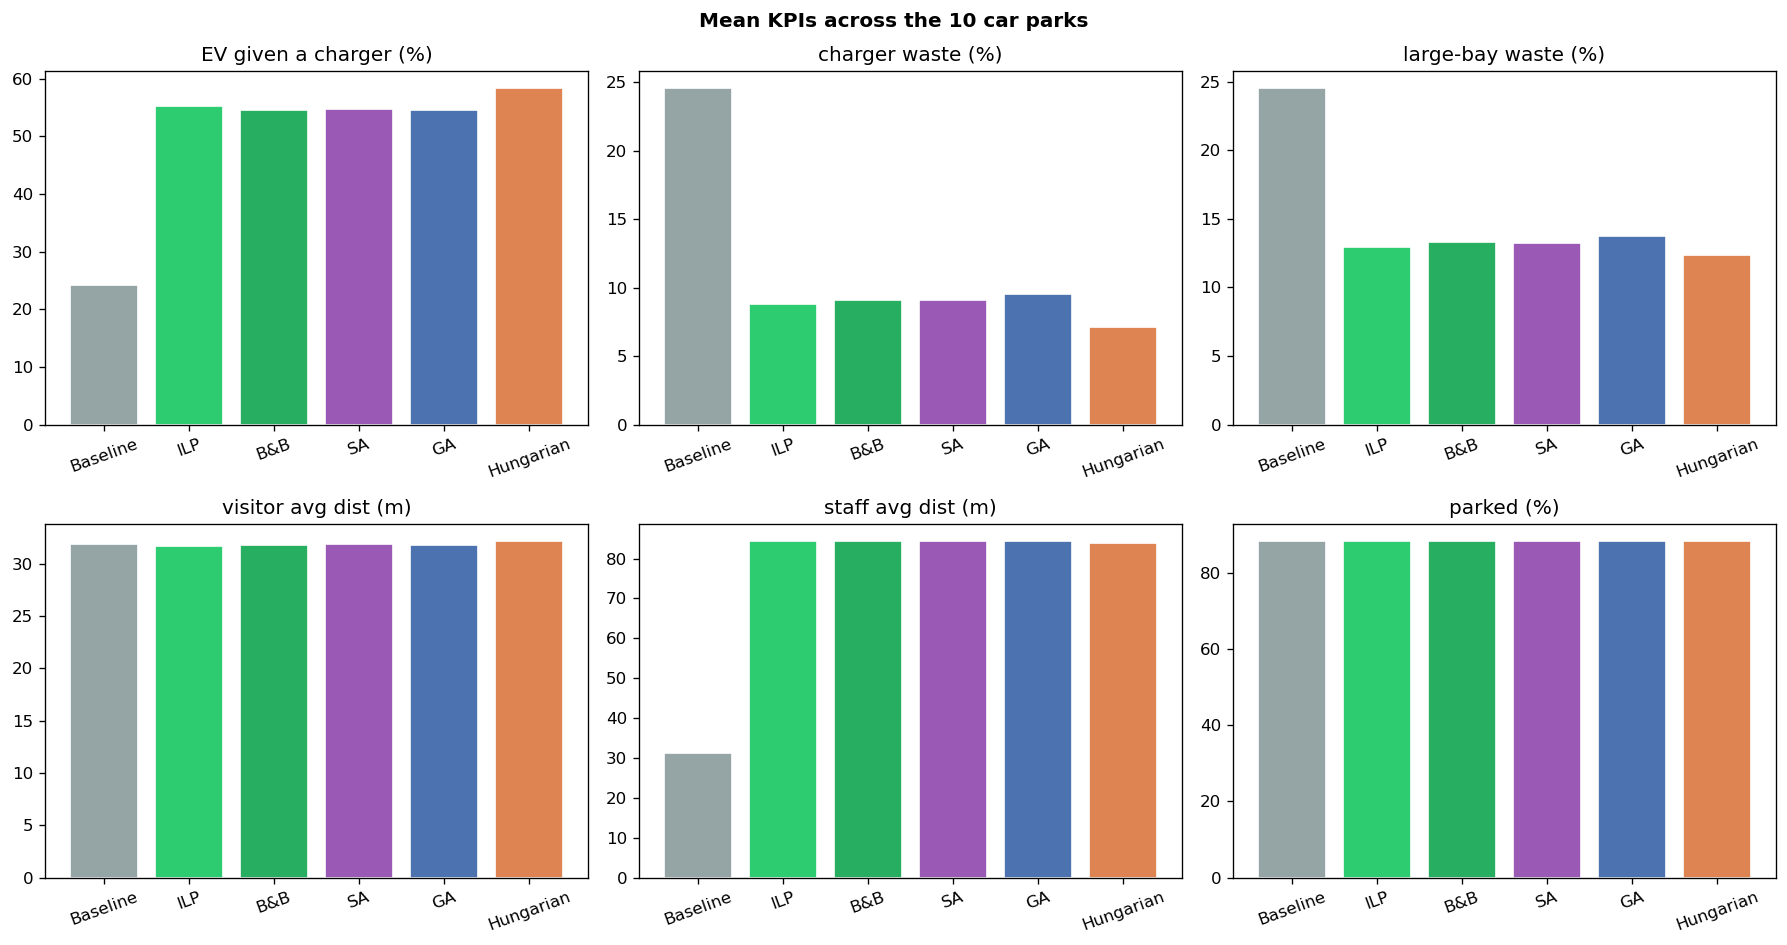
\includegraphics[width=0.95\textwidth]{mt_kpis.png}
  \caption{Mean KPIs across the ten car parks. The naive baseline (grey) is worst on
           every quality metric; Hungarian (orange) leads.}
  \label{fig:kpis}
\end{figure}

\begin{figure}[h]
  \centering
  \begin{subfigure}{0.49\textwidth}
    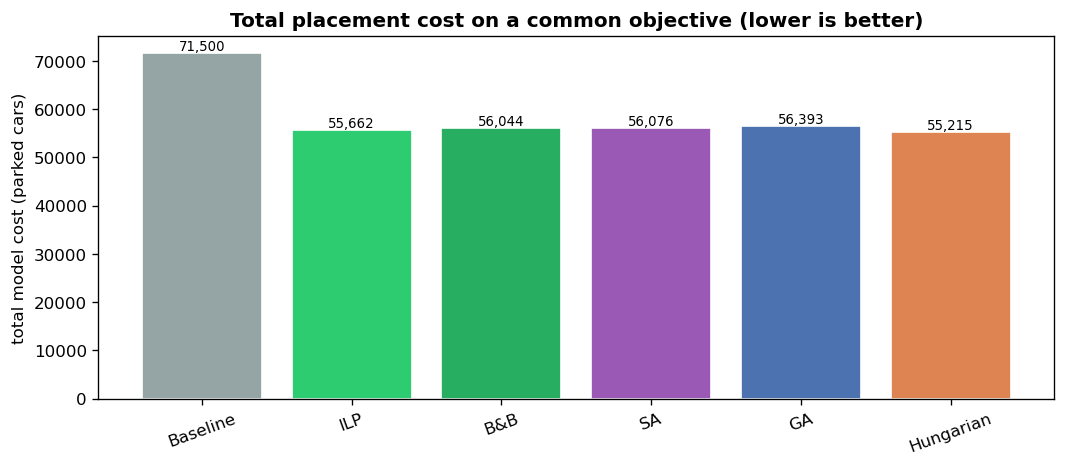
\includegraphics[width=\textwidth]{mt_cost.png}
    \caption{Total placement cost on the common static objective.}
  \end{subfigure}\hfill
  \begin{subfigure}{0.49\textwidth}
    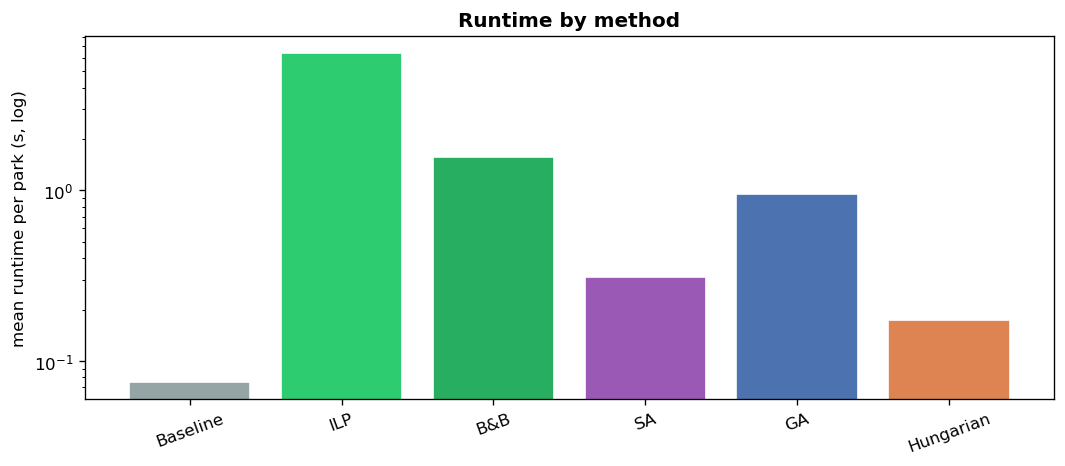
\includegraphics[width=\textwidth]{mt_runtime.png}
    \caption{Mean runtime per park (log scale).}
  \end{subfigure}
  \caption{Cost and runtime. Hungarian achieves the lowest total cost at nearly the speed
           of the baseline; ILP is by far the slowest.}
  \label{fig:cost}
\end{figure}

\begin{figure}[h]
  \centering
  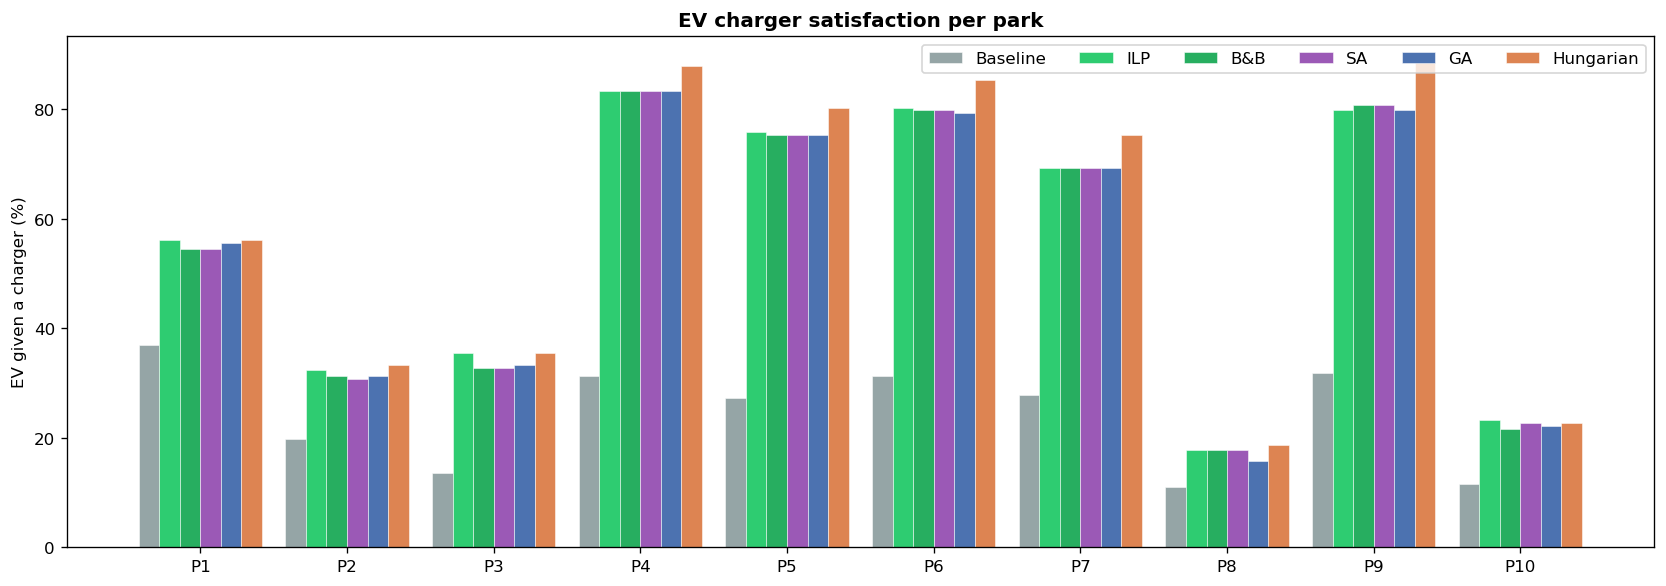
\includegraphics[width=0.95\textwidth]{mt_ev_per_park.png}
  \caption{EV charger satisfaction per park, all six methods. Hungarian leads in almost
           every park; the gap widens where chargers are under pressure.}
  \label{fig:evpark}
\end{figure}

% ============================== 7. INTERPRETATION ==============================
\section{Interpretation}

\subsection{Capacity sets how many park; the method sets how well}

Peak concurrent demand is 355 cars, and three parks cannot hold that. Consequently every
method parks about the same share of cars (around 88\,\%), and the parked-percentage bars
are nearly identical. The interesting differences are not in \emph{how many} cars park
but in \emph{how good} their bays are.

\subsection{Baseline versus the five optimisers}

The naive baseline is far worse on every quality metric. It charges only 24\,\% of EVs
against $\sim$55\,\% for the optimisers; it wastes chargers on non-EVs 25\,\% of the time
against $\sim$9\,\%; it wastes large bays 25\,\% against $\sim$13\,\%; and it parks staff
at 31\,m against $\sim$84\,m. That last figure is the staff flip working: the optimisers
push long-stay staff to the back, the baseline does not. This whole gap is the value of
the scarcity-aware cost together with joint matching. Notice that visitor distance barely
moves ($\sim$32\,m either way): staff are only 51 of 1000 cars, so freeing their bays
helps the 949 visitors only slightly \emph{on average}. The visitor win is qualitative, they keep the prime bays, not a large change in the mean.

\subsection{The exact methods and the metaheuristics tie}

ILP, B\&B, SA and GA all land within about one point of each other. This is expected:
most minutes contain only a few cars, so all four reach the same small per-minute optimum
on the plain cost. ILP is the exact reference; B\&B trails it only because it hits its
time limit on the single 30-car opening minute and returns its warm start there; SA and
GA occasionally miss the exact optimum by a hair. In effect they validate one another.
The practical lesson is that \emph{at this per-minute scale the choice between an exact
method and a good metaheuristic barely matters}, the cost function dominates the
outcome, not the search technique.

\subsection{Hungarian plus anticipation wins, and why}

Hungarian is best on every quality KPI: EV satisfaction 58\,\% (about 3 points above the
exact ILP), the lowest charger waste (7\,\%) and the lowest large-bay waste (12\,\%). The
most instructive comparison is with ILP. ILP is provably optimal \emph{every single
minute}, yet Hungarian ends the day with a \emph{lower total cost on the very same static
objective}. How can a per-minute-optimal method be beaten on the cumulative objective it
optimises?

The answer is that the minutes are \emph{not independent}: a bay given away now is gone
later. ILP minimises only the current minute, so it will hand a charger bay to a non-EV
whenever that is locally cheapest, and then pay the large EV penalty later when an
electric car arrives to find no charger free. Hungarian's anticipation holds those scarce
bays back, so fewer penalties are paid across the whole day, which shows up directly in
its lower charger and large-bay waste. In other words, a per-minute-optimal policy is
still \emph{myopic} in an online setting, and anticipation reduces that myopia. The
important consequence is that anticipation is not trading cost for satisfaction here: it
improves both at once.

\subsection{Runtime}

Runtimes per park (means) are 0.08\,s (Baseline), 0.17\,s (Hungarian), 0.31\,s (SA),
0.96\,s (GA), 1.58\,s (B\&B) and 6.44\,s (ILP). ILP is slowest because it spins up the CBC
solver on every multi-car minute. Hungarian delivers the best quality and the lowest cost
at almost the speed of the baseline, because it is a specialised polynomial algorithm.
This is the practical case for it: best results, near-instant.

\subsection{The weakest lever: floor balancing}

The floor load-balancing term is the least effective component. The distance and charger
pulls toward the lower, nearer floors are far stronger than a weight of 20, so the
optimisers still concentrate cars on the ground and charger floors, and on single-floor
parks the term does nothing at all. It is a tunable constant: raising \code{FLOOR\_LOAD}
would trade walking distance for a more even spread across levels if that ever became the
priority.

% ============================== 8. CONCLUSION ==============================
\section{Conclusion}

Chargers are physically scarce (15 to 77 per park for roughly 198 EVs in the stream), so
no method can charge them all, the ceiling is structural, just as capacity caps the
parked percentage. Within those ceilings, the project shows three clear results. First,
scarcity-aware joint matching roughly \emph{doubles} EV satisfaction over the naive
baseline and \emph{halves} the resource waste, which is the value of the cost function in
Equation~\eqref{eq:cost}. Second, at this per-minute scale the difference between exact
solvers and good metaheuristics is negligible, so a fast specialised method is preferable
to a heavy general one. Third, and most interesting, a history-only anticipation signal
lets the Hungarian method beat the per-minute-optimal ILP on ILP's own cumulative
objective, because it counteracts the myopia inherent in online decision-making. The
recommended configuration is therefore the Hungarian method with anticipation: it gives
the best KPIs and the lowest total cost at near-baseline speed, while fully respecting the
online, unknown-duration, irrevocable nature of the real problem.

\vspace{0.8cm}
\noindent\textbf{Reproducibility.} All results are produced by \code{main.ipynb} run top
to bottom with fixed seeds; figures are written to \code{viz/} and the full per-park KPI
table to \code{viz/mt\_results.csv}.

\end{document}
